\section{大型强子对撞机} \label{sec:LHC}
座落在瑞士法国边境的大型强子对撞机(LHC)是世界目前最大,能量最高的对撞机,其对撞环(储存环)在地下100米,周长为27公里。
%它与之前的大型正负电子对撞机(LEP)使用同样的隧道,并沿用部分加速环。
%LHC可以前所未有的速率及能量提供质子-质子和铅-铅对撞,本文将讨论质子-质子对撞。LHC的质子-质子对撞的设计目标是提供质心系能量为14 TeV,平均瞬时亮度可达
%$10^{34} \text{cm}^{-2}s^{-1}$。关于LHC的详细论述可见~\cite{Evans_2008} \\
在LHC储存环上,有四个相互作用点(实验),分别是ATLAS~\cite{ATLAS_Collaboration_2008},CMS~\cite{CMS_Collaboration_2008},LHCb~\cite{LHCb_Collaboration_2008}以及ALICE~\cite{ALICE_Collaboration_2008},其相对位置如简图~\ref{fig:LHC_schematic}所示。
ALTAS和CMS是多用途探测器,主要为了检验标准模型和发现TeV量级新物理,随后会进一步介绍ATLAS探测器。
LHCb实验主要用于CP破坏以及$b$强子稀有衰变的精确测量。ALICE实验主要研究重离子对撞。
本文将讨论质子-质子对撞和ATLAS实验。
\begin{figure}[h]
\begin{center}
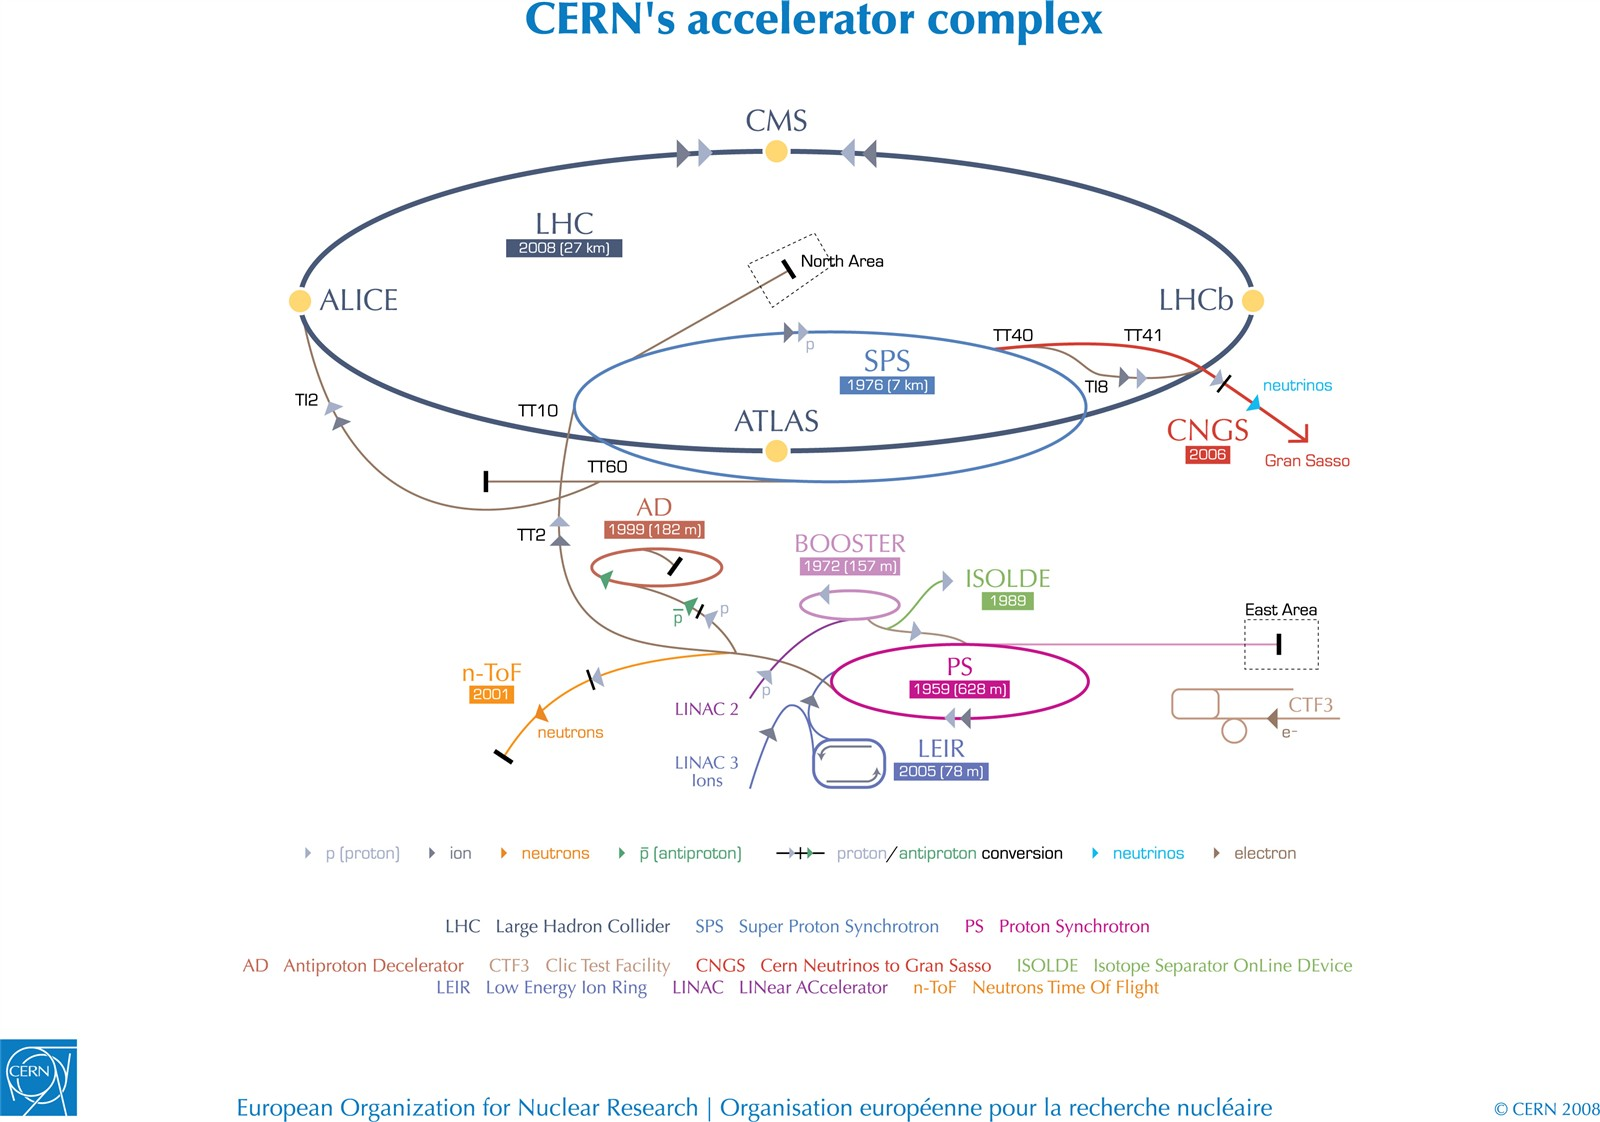
\includegraphics[width = 0.9\textwidth,angle=-90]{fig/LHC-shematic.jpg}
\caption{LHC概览} \label{fig:LHC_schematic}
\end{center}
\end{figure}

\subsection{质子加速过程}
LHC的设计目标是提供质心系能量为14 TeV,平均瞬时亮度可达$10^{34} \text{cm}^{-2}s^{-1}$的质子-质子对撞。
质子来源于电离氢气,而后会经历以下加速过程:
\begin{itemize}
  \item 通过线性加速器(Linac2)加速到50 MeV($\beta\approx5\%$);
  \item 注入到质子同步推进器(Proton Synchrotron Booster),加速至1.4 GeV($\beta\approx70\%$);
  \item 质子同步器(Proton Synchrotron)加速至25 GeV($\beta\approx99.9\%$);
  \item 超级质子同步器(Super Proton Synchrotron)提升至450 GeV($\beta\approx99.9998\%$);
  \item 注入储存环上的两条束流管,一条顺时针,另一条逆时针转圈,每次注入大约花费4分钟。
  \item 最终通过储存上的超导高频腔加速到6.5 TeV。
\end{itemize}
LHC的每次注入可持续几小时,直到束流密度下降到一定阈值,而后,束流被导出,一个新的循环开始。

\subsection{LHC重要参数}
LHC的瞬时亮度公式如下:
\begin{equation}
\mathcal{L}=\frac{N_{b}^{2}f_{r}n_{b}F}{4\pi\varepsilon_{n}\beta^{*}}
\end{equation}
其中$N_b$(束流团所含质子数),$n_b$(储存环中运行束流团数),$f_{r}$(束流团旋转频率)以及$\varepsilon_n$(束团归一横向发射度,描述粒子横向扩散)由质子加速过程决定;
而$\beta^{*}$是在对撞点的所谓振幅函数,它的性质由聚焦磁铁决定;F是为修正束团对撞角度偏差的束流形状因子,一般小于1。$\varepsilon_{n}\beta^{*}$正比于束流横向面积,
那么越小的横向发射度或者越小的振幅函数意味着更窄的束流,对撞频率就越高。关于LHC亮度的重要参数如表~\ref{tab:lhc_run_summary}所示,需要注意的是,自LHC开机以来,一直在进行优化,一些所列
参数已经超过设计指标,比如最大瞬时亮度,其已在2016年运行时超过$10^{34}~\text{cm}^{-2}~\text{s}^{-1}$,主要是因为更小的$\beta^{*}$和优化的形状因子。相应地,pileup数也随之增加,见图\ref{fig:mu_2015_2016}。
2015年到2017年LHC亮度及ATLAS数据收集情况总结在图\ref{fig:}。
\begin{table}[h]
\centering
\begin{tabular}{ccccccc}
\hline
Beam/collision parameters    &2015       &2016  &Nominal design (if available)\\
Center-of-mass energy ($\sqrt{s}$) [TeV]     &13   &13    &14 \\
Bunch spacing [ns]   &50-25   &25    &25 \\
Bunch revolution frequency ($f_{r}$) [kHz]  &11.245  &11.245  &11.245 \\
Max. number of bunches/beam ($n_{b}$)   &2232    &2208    &2808  \\
Max. charge per bunch colliding ($10^{11}~$p/bunch) &1.21   &1.31   &1.15 \\
Peak instantaneous luminosity [$10^{34}~\text{cm}^{-2}~\text{s}^{-1}$]  &0.5  &1.38  &1  \\
Max. pileup  &28.2   &52.2   & \\
Longest stable beams fill duration [h]  &24.3 &37.03  & \\
\hline
\end{tabular}
\caption{LHC设计指标,以及在2015年和2016年的运行参数~\cite{LHC-Run-Summary}}
\label{tab:lhc_run_summary}
\end{table}

\begin{figure}[h]
\centering
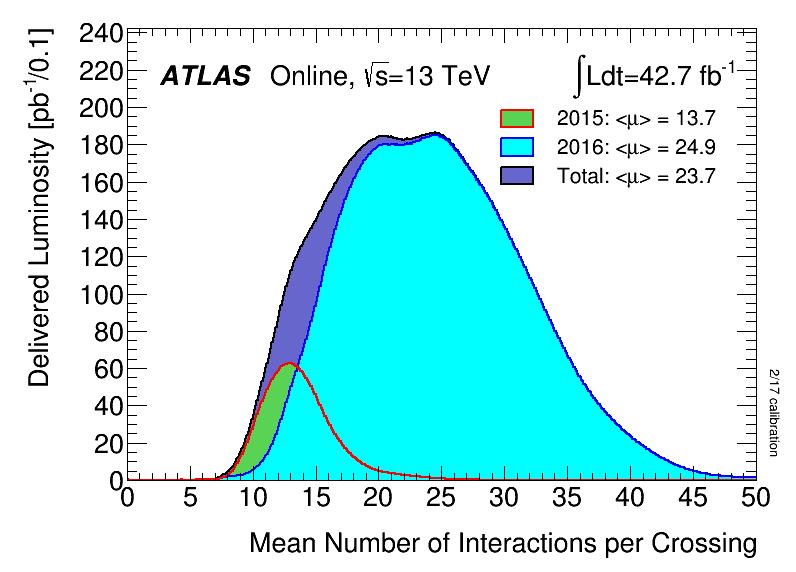
\includegraphics[width = 0.75\textwidth]{fig/mu_2015_2016.png}
\caption{ATLAS 2015年和2016年亮度-pileup分布。}
\label{fig:mu_2015_2016}
\end{figure}
\begin{figure}[!htbp]
    \centering
    \begin{subfigure}[b]{0.45\textwidth}
      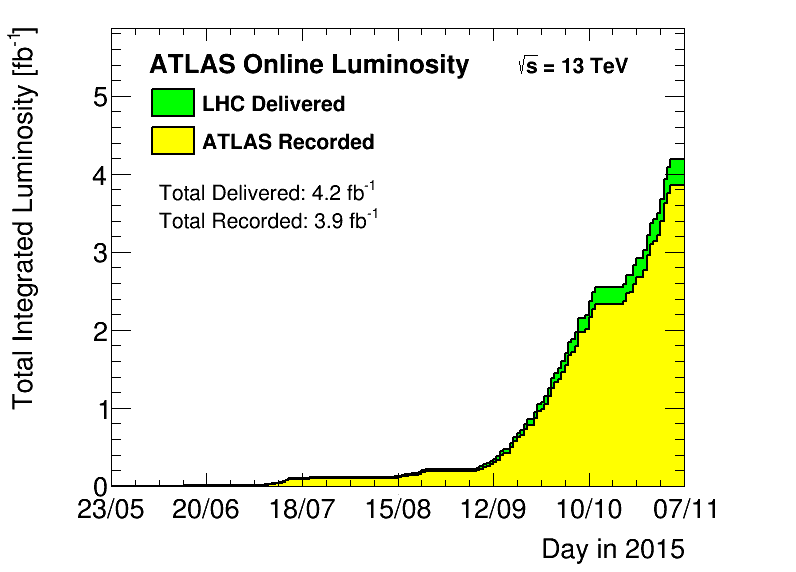
\includegraphics[width=\textwidth]{fig/sumLumiByDay.png}
      \caption{}
      \label{fig:data_taking_2015}
    \end{subfigure}%
    ~%add desired spacing
    \begin{subfigure}[b]{0.45\textwidth}
      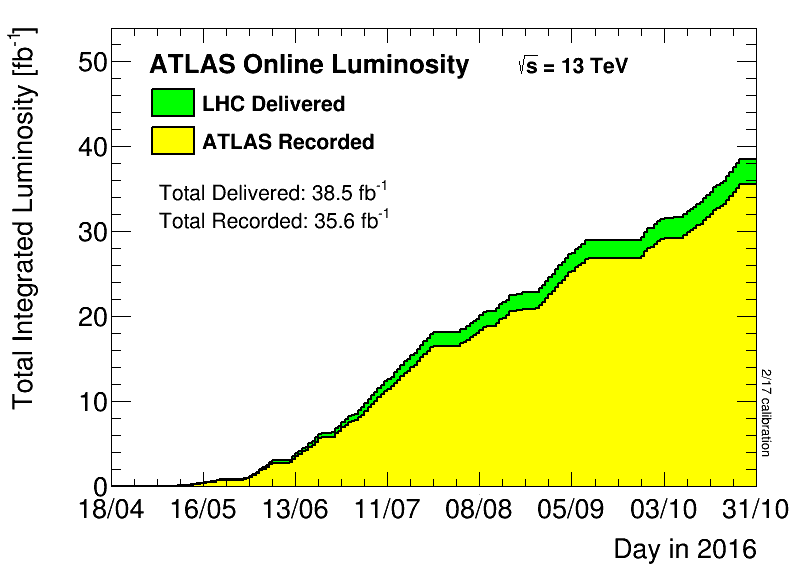
\includegraphics[width=\textwidth]{fig/sumLumiByDay_2016.png}
      \caption{}
      \label{fig:data_taking_2016}
    \end{subfigure} \\
    \begin{subfigure}[b]{0.45\textwidth}
      \centering
      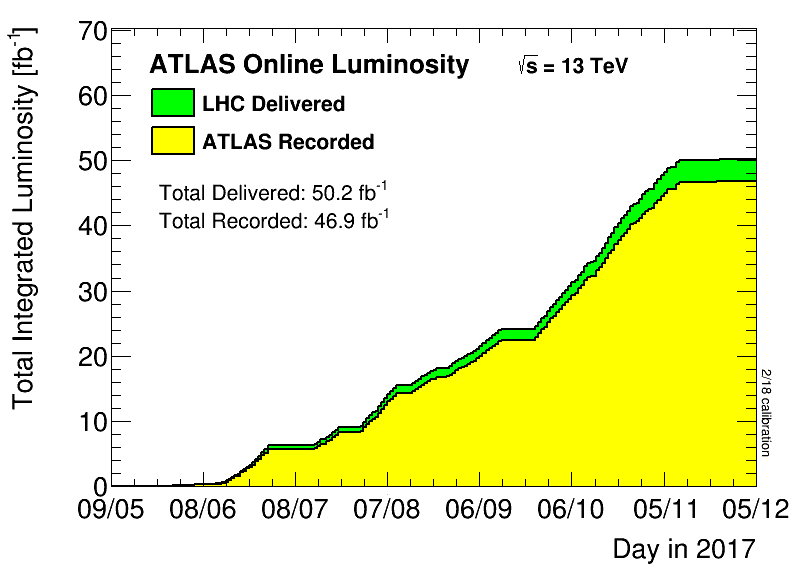
\includegraphics[width=\textwidth]{fig/sumLumiByDay_2017.png}
      \caption{}
      \label{fig:data_taking_2017}
    \end{subfigure}
    \caption{ATLAS数据收集情况: (a)2015年, (b)2016年, (c)2017年。}
    \label{fig:data_taking}
\end{figure}
